\section{Processamento de Linguagem Natural}
\label{s.nlp}

\begin{frame}{Processamento de Linguagem Natural}
	\begin{itemize}
		\justifying	
		\item Quaisquer formas de comunicação, escrita ou verbal, carregam vastas quantias de informação, as quais podem ser utilizadas para \textbf{prever} o comportamento humano;
		\\~\\
		\item Tais informações \textbf{não} são \textbf{triviais} de serem analisadas, pois cada ser humano possui características inerentes à sua forma de comunicação.
	\end{itemize}
\end{frame}

\begin{frame}
	\begin{figure}[!ht]
		\centering
		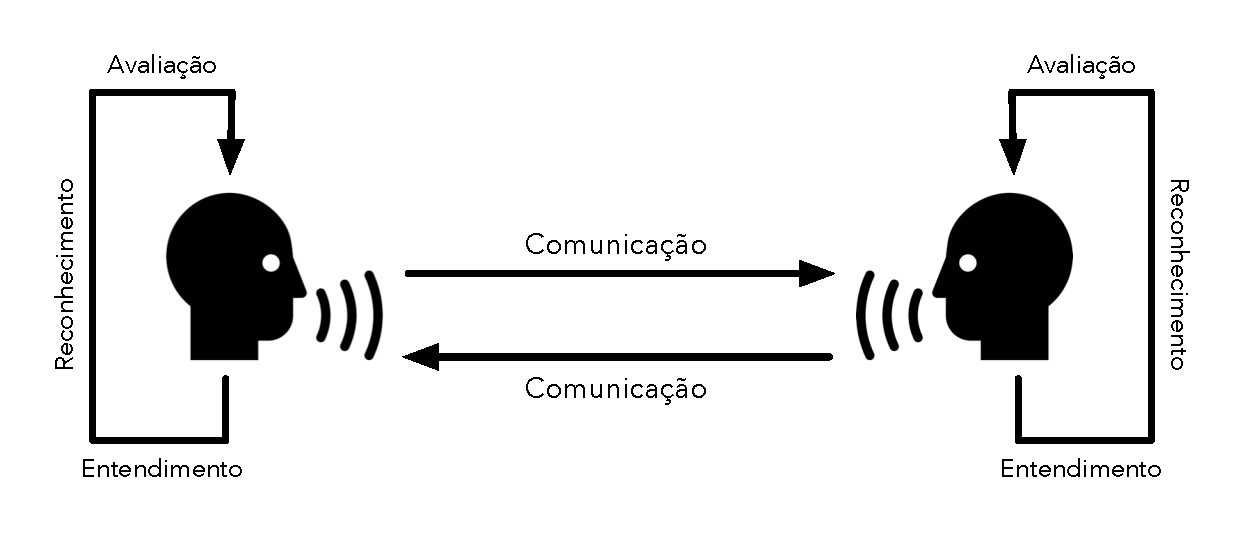
\includegraphics[scale=0.45]{figs/speech_workflow.eps}	
		\label{f.speech_workflow}
		\caption{Processo de comunicação simplificado entre dois seres humanos.}
	\end{figure}
\end{frame}

\begin{frame}
	\begin{itemize}
		\justifying
		\item O objetivo final de um sistema de Processamento de Linguagem Natural é \textbf{compreender e utilizar} uma linguagem da mesma forma que o próprio humano a utiliza;
		\\~\\
		\item Uma compreensão inteligível da linguagem humana requer um \textbf{discernimento} tanto de caracteres como de palavras e, ademais, como ambos estão conectados;
		\\~\\
		\item Enquanto humanos são capazes de aprender e masterizar uma linguagem facilmente, as máquinas ainda esbarram em suas características \textbf{ambíguas} e \textbf{imprecisas}.
	\end{itemize}
\end{frame}

\begin{frame}
	\begin{figure}[!ht]
		\centering
		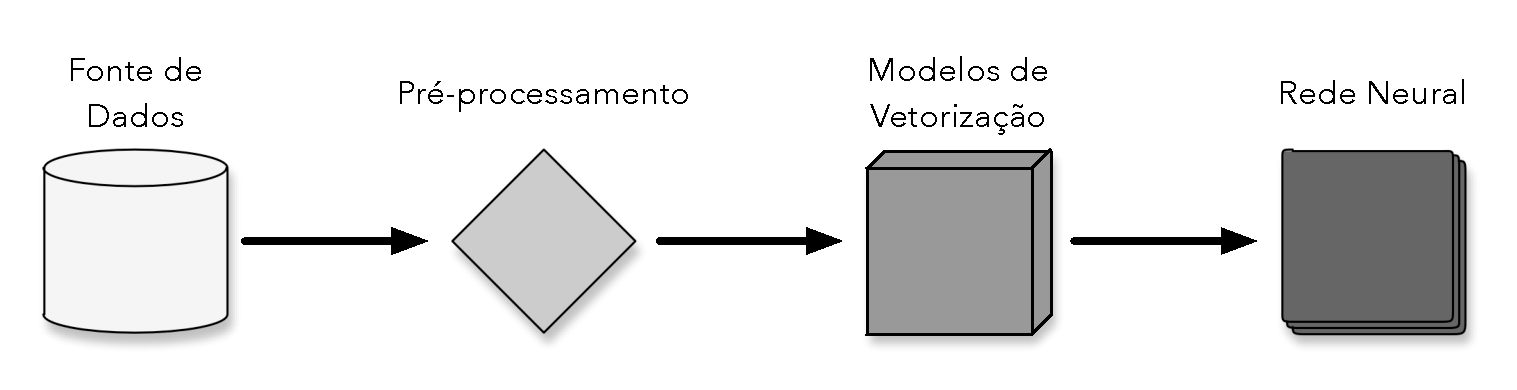
\includegraphics[scale=0.4]{figs/nlp_workflow.eps}	
		\label{f.nlp_workflow}
		\caption{Fluxograma da modelagem de um problema de Processamento de Linguagem Natural.}
	\end{figure}
\end{frame}

\subsection{Exemplos de Tarefas}
\label{ss.tasks}

\begin{frame}{Exemplos de Tarefas}
	\justifying
	\begin{itemize}
		\item Diálogo: Análise de discursos, resolução de correferências e sumarização automática;
		\\~\\
		\item Semântica: Análise de sentimentos, desambiguação de palavras, entendimento de linguagem natural, extração de relacionamentos, \textbf{geração de linguagem natural}, reconhecimento de entidades nomeadas, reconhecimento de vínculo textual, reconhecimento ótico de caracteres, semântica léxica, semântica distribucional, segmentação de tópicos, sistema de perguntas e respostas e tradução de máquina;	
		\end{itemize}
\end{frame}

\begin{frame}
	\justifying
	\begin{itemize}
		\item Sintaxe: Análise gramatical, extração de terminologias, indução gramatical, lematização, marcação de partes da fala, quebra de sentenças, segmentação de palavras, segmentação morfológica e stemização;
		\\~\\
		\item Voz: conversor de texto para voz, reconhecimento de voz e segmentação de voz.
		\end{itemize}
\end{frame}

\begin{frame}
	\begin{figure}[!ht]
		\centering
		
\includegraphics[scale=0.4]{figs/nlp_applications.eps}	
		\label{f.nlp_applications}
		\caption{Exemplos de aplicações baseadas em Processamento de Linguagem Natural. Em sentido horário: \emph{Google Translate}, \emph{Microsoft Word}, \emph{Grammarly}, \emph{Cortana}, \emph{Siri}, \emph{OK Google}, \emph{Alexa} e \emph{IBM Watson}.}
	\end{figure}
\end{frame}

\subsection{Geração de Linguagem Natural}
\label{ss.gln}

\begin{frame}{Geração de Linguagem Natural}
	Lorem ipsum ...
\end{frame}